\documentclass[11pt,]{article}
\usepackage[]{mathpazo}
\usepackage{amssymb,amsmath}
\usepackage{ifxetex,ifluatex}
\usepackage{fixltx2e} % provides \textsubscript
\ifnum 0\ifxetex 1\fi\ifluatex 1\fi=0 % if pdftex
  \usepackage[T1]{fontenc}
  \usepackage[utf8]{inputenc}
\else % if luatex or xelatex
  \ifxetex
    \usepackage{mathspec}
  \else
    \usepackage{fontspec}
  \fi
  \defaultfontfeatures{Ligatures=TeX,Scale=MatchLowercase}
\fi
% use upquote if available, for straight quotes in verbatim environments
\IfFileExists{upquote.sty}{\usepackage{upquote}}{}
% use microtype if available
\IfFileExists{microtype.sty}{%
\usepackage{microtype}
\UseMicrotypeSet[protrusion]{basicmath} % disable protrusion for tt fonts
}{}
\usepackage{hyperref}
\PassOptionsToPackage{usenames,dvipsnames}{color} % color is loaded by hyperref
\hypersetup{unicode=true,
            colorlinks=true,
            linkcolor=black,
            citecolor=black,
            urlcolor=black,
            breaklinks=true}
\urlstyle{same}  % don't use monospace font for urls
\usepackage{natbib}
\bibliographystyle{amnat}
\usepackage{graphicx,grffile}
\makeatletter
\def\maxwidth{\ifdim\Gin@nat@width>\linewidth\linewidth\else\Gin@nat@width\fi}
\def\maxheight{\ifdim\Gin@nat@height>\textheight\textheight\else\Gin@nat@height\fi}
\makeatother
% Scale images if necessary, so that they will not overflow the page
% margins by default, and it is still possible to overwrite the defaults
% using explicit options in \includegraphics[width, height, ...]{}
\setkeys{Gin}{width=\maxwidth,height=\maxheight,keepaspectratio}
\IfFileExists{parskip.sty}{%
\usepackage{parskip}
}{% else
\setlength{\parindent}{0pt}
\setlength{\parskip}{6pt plus 2pt minus 1pt}
}
\setlength{\emergencystretch}{3em}  % prevent overfull lines
\providecommand{\tightlist}{%
  \setlength{\itemsep}{0pt}\setlength{\parskip}{0pt}}
\setcounter{secnumdepth}{0}
% Redefines (sub)paragraphs to behave more like sections
\ifx\paragraph\undefined\else
\let\oldparagraph\paragraph
\renewcommand{\paragraph}[1]{\oldparagraph{#1}\mbox{}}
\fi
\ifx\subparagraph\undefined\else
\let\oldsubparagraph\subparagraph
\renewcommand{\subparagraph}[1]{\oldsubparagraph{#1}\mbox{}}
\fi

%%% Use protect on footnotes to avoid problems with footnotes in titles
\let\rmarkdownfootnote\footnote%
\def\footnote{\protect\rmarkdownfootnote}

%%% Change title format to be more compact
\usepackage{titling}

% Create subtitle command for use in maketitle
\providecommand{\subtitle}[1]{
  \posttitle{
    \begin{center}\large#1\end{center}
    }
}

\setlength{\droptitle}{-2em}

  \title{}
    \pretitle{\vspace{\droptitle}}
  \posttitle{}
    \author{}
    \preauthor{}\postauthor{}
    \date{}
    \predate{}\postdate{}
  
%%% Modified from Latex Template for Am. Nat., many other details aren't necessary because they are specified in YAML header of Rmarkdown document.
\usepackage{fullpage}
\linespread{1.7}
\usepackage{lineno}

% code below is important for holding figure positions in main text. Make sure to set fig.pos="H" in code chunk for figure.
\usepackage{float}
\let\origfigure\figure
\let\endorigfigure\endfigure
\renewenvironment{figure}[1][2] {
    \expandafter\origfigure\expandafter[H]
} {
    \endorigfigure
}

\begin{document}

\vspace*{0.1cm}

\begin{center} \LARGE Loss of consumers constrains phenotypic evolution in the resulting food web \end{center}

\bigskip

\begin{center} \large Matthew A. Barbour$^{1,2,\ast}$, Christopher J. Greyson-Gaito$^{2,3}$, Arezoo Sootodeh$^{2}$, Brendan Locke$^{4}$, Jordi Bascompte$^{1}$ \normalsize \end{center}

\bigskip

\noindent 1. University of Zurich, Department of Evolutionary Biology
and Environmental Studies, Zurich, 8057 ZH, Switzerland;

\noindent 2. University of British Columbia, Department of Zoology,
Vancouver, BC V6T 1Z4, Canada;

\noindent 3. University of Guelph, Department of Integrative Biology,
Guelph, ON N1G 2W1, Canada;

\noindent 4. Humboldt State University, Department of Biological
Sciences, Arcata, CA 95521, USA.

\(^\ast\) Corresponding author; e-mail:
\href{mailto:matthew.barbour@ieu.uzh.ch}{\nolinkurl{matthew.barbour@ieu.uzh.ch}}

\bigskip

\emph{Short Running Title}: Consumer loss constrains phenotypic
evolution

\bigskip

\emph{Keywords}: adaptive landscape, ecological networks,
eco-evolutionary dynamics, natural selection, host-parasitoid,
complexity, biodiversity, community context.

\bigskip

\emph{Abstract Word Count}: 251

\bigskip

\emph{Total Word Count}: 5769

\bigskip

\emph{Manuscript type}: Letter.

\bigskip

\linenumbers{} \modulolinenumbers[3]

\newpage

\section{Abstract}\label{abstract}

The loss of biodiversity is altering the structure of ecological
networks; however, we are currently in a poor position to predict how
these altered communities will affect the evolutionary potential of
remaining populations. Theory on adaptive landscapes provides a
framework for predicting how selection constrains phenotypic evolution,
but often treats the network context of evolving populations as a
``black box''. Here, we integrate ecological networks and adaptive
landscapes to examine how changes in food-web structure shape
evolutionary constraints. We conducted a field experiment that removed a
guild of larval parasitoids that imposed direct and indirect selection
pressures on an insect herbivore. We then measured herbivore survival as
a function of three key phenotypic traits to estimate directional,
quadratic, and correlational selection gradients in each treatment. We
used these selection gradients to characterize the slope and curvature
of the adaptive landscape to understand the direct and indirect effects
of consumer loss on evolutionary constraints. We found that the number
of traits under directional selection increased with the removal of
larval parasitoids, indicating greater selective constraints on the
trajectory of evolutionary change. Similarly, we found that the removal
of larval parasitoids altered the curvature of the adaptive landscape in
such a way that tended to decrease the evolvability of the traits we
measured in the next generation. Our results suggest that the loss of
trophic interactions can impose greater constraints on phenotypic
evolution. This indicates that the simplification of ecological
communities may constrain the adaptive potential of remaining
populations to future environmental change.

\newpage

\section{Impact Summary}\label{impact-summary}

The loss of biodiversity is rewiring the web of life; however, it is
uncertain how this will affect the ability of remaining populations to
evolve and adapt to future environments. To gain insight to these
effects, we conducted a field experiment that either maintained a
natural community of predators or removed all but one of the predators
that was able to impose selection on a common prey. We found that the
loss of predators acted to constrain prey evolution toward a particular
combination of traits. Moreover, we found that the loss of predators
could make it more difficult for prey to adapt to uncertain future
environments. Taken together, our results suggest that the
simplification of the web of life may constrain the adaptive potential
of remaining populations.

\newpage

\section{Introduction}\label{introduction}

The adaptive landscape provides a powerful framework for understanding
how natural selection has shaped the evolution of biodiversity ---from
genes to phenotypes to species
\citep{Wright1931, Simpson1944, Arnold2001}. More than a metaphor, the
adaptive landscape links quantitative genetic and phenotypic variation
to evolution by natural selection
\citep{Lande1979, Arnold1984applications, Arnold1984theory}, giving
insight to the direct and indirect effects of selective constraints
\citep{Arnold1992}. Ecological interactions often play a key role in
shaping selective constraints, as evidenced by the role of antagonistic
and mutualistic interactions in driving evolutionary change
\citep{Schluter2000, Abrams2000, Bronstein2006}. Although there is clear
evidence that species interactions can shape the adaptive landscape, we
still have a poor understanding of how the adaptive landscape is shaped
by a community of interacting species \citep{McPeek2017, terHorst2018}.
Resolution on how change in ecological communities shape phenotypic
evolution is urgently needed though, given the rapid losses of
biodiversity we are observing in the Anthropocene \citep{Scheffers2016}.

Ecological networks, such as food webs describing who-eats-whom, provide
an explicit representation of the direct and indirect effects that
emerge in a community of interacting species
\citep{Bascompte2014, McCann2012}. Here, we integrate ecological
networks and adaptive landscapes to understand how ecological
communities constrain evolutionary change. The direct and indirect
effects of natural selection can be inferred by quantifying the slope
and curvature of the adaptive landscape \citep{Arnold1992}. For example,
the slope is determined by directional selection gradients acting on
each phenotypic trait and influences the trajectory of evolutionary
change \citep{Lande1979, Arnold1992}. Selective constraints on evolution
increase with the number of traits under directional selection, as this
diminishes the number of optimal solutions \citep{Arnold2003}. The
curvature of the adaptive landscape is governed by nonlinear selection
gradients and acts to indirectly constrain evolution through its effect
on genetic constraints \citep{Arnold1992, Hansen2008}. Genetic
constraints are largely governed by a population's \textbf{G}-matrix
---the additive genetic variances and covariances between traits
\citep{Hansen2008}. Stabilizing selection acts to erode genetic variance
in traits, which can impose a constraint on the ability of those traits
to respond to future selection \citep{Hansen2008}. Correlational
selection may alter the genetic covariance between traits, which may
facilitate or hinder future adaptation depending on pattern of selection
on those traits \citep{Hansen2008}. If we want to predict how ecological
communities shape phenotypic evolution, we must understand how
ecological networks shape the adaptive landscape.

The loss of biodiversity is altering the structure of ecological
networks, which may influence evolutionary constraints in a number of
ways. For example, in a food web, if different consumers impose
directional selection on different traits of a shared resource, then a
more diverse consumer community may constrain evolution by increasing
the number of traits under selection. Alternatively, if consumers impose
selection on different values of a trait, then their selective effects
would cancel each other out in more diverse communities. To examine
these different possibilities, we conducted a field experiment that
removed a consumer guild that directly and indirectly impacts fitness of
an abundant insect herbivore (\emph{Iteomyia salicisverruca}, Family
Cecidomyiidae; fig. \ref{fig:Conceptual}). The larvae of this herbivore
induce tooth-shaped galls when they feed on the developing leaves of
willow trees \citep[\emph{Salix} sp.,][]{Russo2006}. These galls protect
larva from attack by generalist predators (e.g.~ants, spiders), but they
suffer high mortality from egg and larval parasitoids
\citep{Barbour2016}. We manipulated food-web structure by either
removing larval parasitoids (removal food web) or allowing both egg and
larval parasitoids to impose selection on gall midge traits (original
food web, fig. \ref{fig:Conceptual}). The relative abundance of these
larval parasitoids is much lower than the egg parasitoid
\citep{Barbour2016}, and thus represents a plausible extinction scenario
for this system. Larval parasitoids also impose indirect effects on gall
midge fitness through intraguild predation on the egg parasitoid (fig.
\ref{fig:Conceptual}). We applied modern statistical methods to quantify
how changes in food-web structure altered the slope and curvature of the
gall midge's adaptive landscape. Taken together, our study gives insight
to how the loss of biodiversity may constrain the evolution of
interacting populations.

\begin{figure}
\centering
\includegraphics{../analyses/complex_simple_foodwebs_v3.jpeg}
\caption{\label{fig:Conceptual}Experimental manipulation of food-web
structure associated with a leaf-galling midge (\emph{Iteomyia
salicisverruca}) feeding on the willow \emph{Salix hookeriana}. Black
arrows denote the flow of energy in this network of trophic
interactions. In the original food web, we allowed the full suite of egg
and larval parasitoids to impose selection. In the removal food web, we
used mesh bags to exclude the guild of larval parasitoids, only allowing
the egg parasitoid (\emph{Platygaster} sp.) to impose selection. Note
that larval parasitoids also impose indirect effects on gall midge
fitness through intraguild predation on the egg parasitoid. Larval
parasitoids include the following species (from left to right):
\emph{Mesopolobus} sp. (Family: Pteromalidae); \emph{Tetrastichus} sp.
(Family: Eulophidae); and \emph{Torymus} sp. (Family: Torymidae).}
\end{figure}

\section{Methods}\label{methods}

\subsection{Study Site}\label{study-site}

We conducted our study within a four-year old common garden experiment
of coastal willow (\emph{Salix hookeriana}) located at Humboldt Bay
National Wildlife Refuge (HBNWR) (40 40'53``N, 124 12'4''W) near Loleta,
California, USA. This common garden consists of 26 different willow
genotypes that were collected from a single population of willows
growing around Humboldt Bay. Stem cuttings of each genotype (25
replicates per genotype) were planted in a completely randomized design
in two hectares of a former cattle pasture at HBNWR. Willows at our
study site begin flowering in February and reach their peak growth in
early August. During this study, willows had reached 5 - 9m in height.
Further details on the genotyping and planting of the common garden are
available in \citet{Barbour2015}.

\subsection{Manipulating Food-web
Structure}\label{manipulating-food-web-structure}

We setup our food-web manipulation across 128 plants soon after galls
began developing on willows in early June of 2013. These 128 plants came
from eight different plant genotypes that spanned the range of trait
variation observed in this willow population \citep{Barbour2015}. For
the original food web (eight replicates per genotype), we used flagging
tape to mark 14 galled leaves per plant (\textasciitilde{}30 larvae),
allowing the full suite of egg and larval parasitoids to impose
selection. Marking galls with flagging tape ensured that all galls had
similar phenology when we collected galls later in the season. For the
removal food web, we enclosed 14 galled leaves with 10x15cm organza bags
(ULINE, Pleasant Prairie, WI, USA) to exclude three parasitoid species
that attack during larval development. This treatment did not exclude
the egg parasitoid \emph{Platygaster} sp., which attacks prior to gall
initiation \citep[larva initiate gall development in Cecidomyiid
midges:][]{Gagne1989}. It was not possible to reciprocally manipulate
parasitoid attack (i.e.~exclude egg parasitoid, but allow larval
parasitoids), because it was not possible to identify midge oviposition
sites prior to gall formation. In late August, we collected marked and
bagged galls from each plant, placed them into 30 mL vials and kept them
in the lab for 4 months at room temperature. We then opened galls under
a dissecting scope and determined whether larvae survived to pupation
(our measure of fitness) or were parasitized. We did not include other
sources of mortality, such as early larval death, as they could
influence the expression of the gall phenotype and confound estimates of
selection. For the food-web treatment that excluded larval parasitoids,
we further restricted our data by removing any incidental instances of
parasitism by a larval parasitoid. This represented less than 3\% of the
observations in this food-web treatment and allowed us to focus our
inferences of selection on those imposed by the egg parasitoid. Our
final dataset contains survival estimates for 1285 larvae from 613 galls
and 111 plants.

\subsection{Measuring Phenotypic
Traits}\label{measuring-phenotypic-traits}

We collected data on three different traits that we expected to
influence larval survival based on previous work in this system
\citep{Barbour2016} and other work with gall midges
\citep{Weis1983, Heath2018}. First, we measured gall diameter as the
size of each gall chamber to the nearest 0.01 mm at its maximum diameter
(perpendicular to the direction of plant tissue growth). Previous work
in this system has shown that larger galls are associated with higher
survival \citep{Barbour2016}. Second, we measured clutch size by
counting the number of chambers in each gall
\citep{Weis1983, Heath2018}. All larvae collected from the same
multi-chambered gall were scored with the same clutch size. Third, we
measured oviposition preference as the density of larvae observed on a
plant in an independent survey. We did this by randomly sampling five
branches per tree and counting the number of individual gall chambers
(number of larvae). We then converted these counts to a measure of
larval density per 100 shoots by counting the number of shoots on the
last branch we sampled. All larvae collected from the same plant were
scored with the same oviposition preference. Measuring larval densities
on plants in the field is a common method for measuring oviposition
preference \citep{Gripenberg2010}; however, caution must be taken in
inferring `preference' as larval densities can be influenced by
processes other than preference \citep{Singer1986}. Fortunately, a
couple features of our study system suggest that larval densities may be
a good proxy for oviposition preference. For example, since our data
comes from a randomized placement of plant genotypes in a common garden,
there is no consistent bias in which plant genotypes females are exposed
to while searching for oviposition sites. Also, egg predation is a minor
source of mortality for galling insects in general \citep{Hawkins1997};
therefore, we do not expect any prior egg predation to bias our
estimates of observed larval densities.

\subsection{Quantifying the Adaptive
Landscape}\label{quantifying-the-adaptive-landscape}

Inferring adaptive landscapes assumes that trait distributions are
multivariate normal \citep{Lande1983}. To approximate this assumption,
we log-transformed clutch size and square-root transformed oviposition
preference. We then scaled all phenotypic traits (mean=0 and SD=1)
across treatments prior to our analyses (detailed below) to ensure that
our estimates of selection were comparable across traits and with other
studies.

Our analysis consisted of four parts. First, we used generalized linear
mixed models (GLMM) to quantify selection surfaces \textemdash linear
and nonlinear relationships between absolute fitness (\(W\)) and
standardized phenotypic traits (\(i\)) of individuals \textemdash in
each food-web treatment. Second, we translated selection surfaces into
the scale of relative fitness (\(w\)) in order to calculate standardized
selection gradients. Third, we used our estimates of directional
selection gradients to characterize the slope of the adaptive landscape,
which we used to measure selective constraints. Finally, we estimated
the curvature of the adaptive landscape and used a simulation to explore
its effects on the adaptive potential of the gall midge population in
the next generation.

\textbf{Selection surfaces}: Since larval survival was our measure of
absolute fitness, we used a GLMM that assumed a binomial error
distribution (and logit-link function). To approximate the selection
surface, we modelled larval survival as a function of food-web treatment
as well as linear (\(\alpha_i\)), quadratic (\(\alpha_{ii}\)), and
linear interactions (\(\alpha_{ij}\)) between each trait. We also
allowed these selection surfaces (\(\alpha\)) to vary between food-web
treatments. Note that to obtain valid estimates of linear selection
surfaces, we removed nonlinear terms prior to estimating linear
relationships \citep{Lande1983}. Other approaches have been advocated
for approximating selection surfaces \citep{Schluter1988}; however, our
approach enables us to calculate selection gradients, and thus is more
appropriate for approximating the adaptive landscape \citep{Arnold2003}.
To account for the nonindependence of clutch size (measured at gall
level) and oviposition preference (measured at plant level) as well as
any independent effects of willow genotype on larval survival, we
modelled gall ID nested within plant ID nested within genotype ID as
random effects. Although statistical models with random effects are not
common in analyses of natural selection, we think that modelling random
effects can mitigate biased estimates of selection due to environmental
covariances between traits and fitness \citep{Rausher1992}. Since our
end goal was to characterize the relationship between mean trait values
and mean fitness (adaptive landscape), we assumed the mean value of our
random effects (i.e.~setting them to zero) when calculating selection
surfaces. We then used parametric bootstrapping (1,000 replicates) to
estimate the effect of food-web treatment on larval survival as well as
selection surfaces in each food-web treatment. To determine whether
trait-fitness relationships differed between food-web treatments, we
calculated the difference in bootstrapped replicates between treatments.

\textbf{Selection gradients}: Selection gradients cannot be estimated
directly from GLMMs of selection surfaces because the response is in
terms of absolute fitness and the coefficients are on a nonlinear scale.
For example, the coefficients in the above model measure the change in
the logarithm of the odds of surviving (i.e.
\(\text{ln}\{W(z)/[1-W(z)]\}\)) associated with 1 SD change in a trait
with all other traits held fixed at their mean. Therefore, we used the
method developed by \citet{Janzen1998} to translate selection surfaces
from the above model into the scale of relative fitness in order to
calculate directional (\(\beta_i\)), quadratic (\(\gamma_{ii}\)), and
correlational (\(\gamma_{ij}\)) selection gradients. Briefly, this
method calculates the average gradient of selection surfaces by
multiplying the average of \(W(z)[1-W(z)]\) by each regression
coefficient (e.g. \(\alpha_i\), \(\alpha_{ii}\), or \(\alpha_{ij}\)). We
then divided this average gradient by the mean fitness (\(\bar W\)) to
put it on the scale of relative fitness, and thus interpretable as a
selection gradient. We estimated selection gradients separately for each
food-web treatment. We also determined whether selection gradients
differed between food-web treatments by calculating the difference in
bootstrapped replicates between treatments. Note that we doubled all
quadratic terms prior to calculating selection gradients to put them on
the same scale as estimates of directional and correlational selection
\citep{Stinchcombe2008}.

\textbf{Selective constraints}: The number of selective constraints is
determined by the slope of the adaptive landscape, which in our study
corresponds to:

\[\textbf{Slope} = \begin{pmatrix} \beta_{\text{Diam}} \\ \beta_{\text{Clutch}} \\ \beta_{\text{Pref}} \end{pmatrix} \]
where each \(\beta_i\) corresponds to the directional selection gradient
acting on each trait. By comparing the number of directional selection
gradients that show clear evidence of contributing to the slope
(i.e.~95\% CI does not overlap zero) in our food-web treatments, we can
infer the effect of food-web structure on selective constraints. This
gives insight as to whether there is a specific combination of
phenotypes favored by natural selection (i.e.~more traits under
directional selection), or whether multiple trait combinations have
comparable fitness (i.e.~less traits under directional selection).

\textbf{Genetic constraints}: The indirect effects of selection on the
G-matrix
(\(\Delta\text{G}=\text{G}(\gamma - \beta \beta^\text{T})\text{G}\)) are
governed by the curvature of the adaptive landscape
(\(\text{C}=\gamma - \beta \beta^\text{T}\)), which in our study
corresponds to:

\[\textbf{Curvature} = \begin{pmatrix} \gamma_{\text{Diam:Diam}}&& \\ \gamma_{\text{Clutch:Diam}}&\gamma_{\text{Clutch:Clutch}}& \\ \gamma_{\text{Pref:Diam}} & \gamma_{\text{Pref:Clutch}} &\gamma_{\text{Pref:Pref}} \end{pmatrix} - \begin{pmatrix} \beta_{\text{Diam}}\beta_{\text{Diam}}&& \\ \beta_{\text{Clutch}}\beta_{\text{Diam}}&\beta_{\text{Clutch}}\beta_{\text{Clutch}}& \\ \beta_{\text{Pref}}\beta_{\text{Diam}} & \beta_{\text{Pref}}\beta_{\text{Clutch}} &\beta_{\text{Pref}}\beta_{\text{Pref}} \end{pmatrix}\]

where each \(\gamma_{ii}\) (diagonal) corresponds to the quadratic
selection gradient acting on a trait, and each \(\gamma_{ij}\)
(off-diagonal) corresponds to the correlational selection gradient
acting on a particular trait combination. Note that we ommitted the
upper triangle of each matrix for clarity since it is simply the
reflection of the lower triangle. Subtracting these two matrices results
in the curvature matrix of the adaptive landscape:

\[\textbf{Curvature} = \begin{pmatrix} \text{C}_{\text{Diam:Diam}}&& \\ \text{C}_{\text{Clutch:Diam}} & \text{C}_{\text{Clutch:Clutch}} & \\ \text{C}_{\text{Pref:Diam}} & \text{C}_{\text{Pref:Clutch}} & \text{C}_{\text{Pref:Pref}} \end{pmatrix}\]
where each \(\text{C}_{ii}\) (diagonal) represents the effect of
selection on the additive genetic variance in a trait, and each
\(\text{C}_{ij}\) (off-diagonal) represents the effect of selection on
the additive genetic covariance between a particular trait combination.
We used bootstrapped values of each selection gradient to estimate the
curvature of each component of the matrix and its associated 95\% CI. We
also used this information to determine whether the curvature of each
component differed between our food-web treatments.

Knowledge of the curvature matrix alone gives an incomplete picture of
its indirect effect on genetic constraints. This is because genetic
constraints are ultimately determined by the structure of the G-matrix,
and therefore also depend on its structure before selection. Although we
do not know the underlying G-matrix for the traits we measured in this
experiment, we can still gain insight to how our food-web treatment
would alter genetic constraints more generally. Specifically, we
calculated how our best estimate of the curvature matrix (mean values)
in each treatment changed the structure of \ensuremath{10^{4}} random
G-matrices for the next generation. We restricted the range of additive
genetic variance (\emph{V\textsubscript{G}}) in these G-matrices to
between 0 and 0.5 to reflect typical ranges in narrow-sense heritability
values (\emph{h}\textsuperscript{2}; note that
\emph{h}\textsuperscript{2} = \emph{V\textsubscript{G}} when the
phenotypic variance is scaled to 1). Note that this analysis assumes
that the effects of recombination and mutation on the G-matrix are much
smaller than the effects of selection, which appears to be a reasonable
assumption over short time scales \citep{Arnold2008}.

The G-matrix itself is a complex structure, but has a clear theoretical
link to the evolvability of phenotypic traits \citep{Hansen2008}.
Evolvability measures the ability for a trait to evolve toward a given
direction of selection \citep{Hansen2008}. In the absence of knowledge
about the direction of selection that a population will actually
experience in the next generation, we can compute its average
evolvability over random selection gradients
\citep{Hansen2008, Melo2015}. By computing the average evolvability
(here, we used 1000 random \(\beta\)s) for each of \ensuremath{10^{4}}
random G-matrices, we can then assess how changes in the curvature
matrix alter the evolutionary potential of the associated traits. We
report the distribution of these effect sizes, rather than conduct a
statistical test, because the number of replicates in a simulation can
be arbitrarily high, thus making any effect size statistically
significant \citep{White2014}.

\subsection{Adjusting for biased measurements of
selection}\label{adjusting-for-biased-measurements-of-selection}

Rather than imposing selection, parasitoids may influence the expression
of herbivore traits which could bias measurements of selection. In our
system, it was plausible that parasitoids may influence chamber diameter
by altering larval feeding behavior or killing larvae before they
complete their development. To estimate this potential bias, we subset
our data to only include galls where there was variation in larval
survival within the same gall (i.e.~1 \textgreater{} mean survival
\textgreater{} 0). If we assume that larvae within each gall should have
similar chamber diameters because they come from the same clutch and
experience the same local environment (an assumption our data supports:
gall ID explains 54\% of the variance in chamber diameter), then the
relationship between chamber diameter and larval survival in this data
subset represents the effect of parasitism on trait expression
(i.e.~bias). We used a GLMM with the same structure as described
previously except that we modeled only a linear relationship between
chamber diameter and larval survival (\(\alpha_{\text{Diam}}\)). We
detected a positive bias in both food-web treatments (original
\(\alpha_{\text{Diam}}\)= 0.36 {[}0.05, 0.67{]}; removal
\(\alpha_{\text{Diam}}\)= 0.42 {[}0.01, 0.82{]}), indicating that
unadjusted relationships would overestimate the strength of selection on
chamber diameter. To account for this bias, we substracted our mean
estimates of bias from our estimates with the full dataset prior to
calculating chamber diameter's selection surface and directional
selection gradient.

\subsection{Measuring selection on egg
parasitoids}\label{measuring-selection-on-egg-parasitoids}

Once parasitized, the gall phenotype becomes the phenotype of the egg
parasitoid. This phenotype may influence the egg parasitoid's survival
in the face of larval parasitoids, and thus experiences selection. Our
food-web manipulation allows us to measure selection imposed by larval
parasitoids on the phenotype of egg parasitoids. Using the same models
as described above, we substituted egg parasitism as our response
variable to quantify selection surfaces and selection gradients acting
on the egg parasitoid. Note that we cannot test the effect of food-web
structure on the egg parasitoid's adaptive landscape ---we can only
estimate selection imposed by larval parasitoids. This comparison is
still useful though in determining the extent to which the loss of
consumers may have indirect evolutionary effects by altering selection
on multiple interacting populations.

All analyses and visualizations were conducted in R \citep{R2018}.
Unless otherwise noted, we report mean estimates of selection surfaces
and selection gradients with 95\% confidence intervals in brackets. Note
that for visualizing the adaptive landscape we restrict trait axes to
\(\pm 1\) SD of the mean trait value. This emphasizes the fact that we
can only reliably estimate the shape of the adaptive landscape near the
mean phenotype of the population \citep{Arnold2001}. We also plot mean
larval survival on a natural log scale to accurately reflect the
mathematical definition of the adaptive landscape \citep{Arnold2003}.
All data and code to reproduce the reported results are publicly
available on GitHub
(\url{https://github.com/mabarbour/complexity_selection}) and have been
archived on Zenodo (\url{https://zenodo.org/badge/latestdoi/108833263}).

\section{Results}\label{results}

\subsection{Consumer loss increases selective
constraints}\label{consumer-loss-increases-selective-constraints}

\indent We found that the removal of larval parasitoids increased the
number of gall midge traits under directional selection (3 of 3)
relative to the original food web (1 of 3)(table \ref{Table:Gradients}).
For example, we observed directional selection for smaller clutch sizes
when we excluded larval parasitoids, but there was no evidence of
selection acting on this trait in the original food web (table
\ref{Table:Gradients}; fig. \ref{fig:UV_Landscape}C). This absence of
selection appeared to be a result of conflicting selection pressures
imposed by each guild of parasitoids. Specifically, when we subset our
data to focus on differences between parasitoid guilds, we found that
larval parasitoids actually impose directional selection for larger
clutch sizes (larval parasitoids \(\beta_{\text{Clutch}}\)= 0.13
{[}0.04, 0.24{]}). This conflicting selection is likely due to trait
differences between guilds, as larger clutches may be easier targets for
egg parasitoids to find, but the more complex gall structure may be more
difficult for larval parasitoids to oviposit through.

\bigskip

\begin{table}[h]
\caption{Standardized selection gradients acting on gall midges in the original food web and with the removal of larval parasitoids.}
\label{Table:Gradients}
\centering
\begin{tabular}{lccc}
\\ 
\hline
\textbf{Selection gradient} & \textbf{Original} & \textbf{Removal} & \textbf{Contrast} \\
\hline
$\beta_{\text{Diam}}$ & 
\textbf{
0.34 [
0.22,
0.48] } & 
\textbf{
0.21 [
0.12,
0.31] } & 
\textbf{
0.14 [
0.27,
0] }\\

$\beta_{\text{Clutch}}$ & 
0.06 [
-0.05,
0.17] & 
\textbf{
-0.09 [
-0.17,
-0.01] } & 
\textbf{
0.15 [
0.29,
0.03] }\\

$\beta_{\text{Pref}}$ &
-0.13 [
-0.29,
0.05] & 
\textbf{
-0.16 [
-0.26,
-0.06] } & 

0.03 [
0.21,
-0.15] \\

$\gamma_{\text{Diam:Diam}}$ &
0.13 [
-0.06,
0.33] & 

0.1 [
-0.02,
0.23] & 

0.03 [
0.27,
-0.2] \\

$\gamma_{\text{Clutch:Clutch}}$ & 
-0.05 [
-0.27,
0.18] & 

-0.11 [
-0.28,
0.03] & 

0.06 [
0.32,
-0.2] \\

$\gamma_{\text{Pref:Pref}}$ & 
\textbf{
0.34 [
0.07,
0.63] }& 

0.02 [
-0.15,
0.18] & 
\textbf{
0.32 [
0.64,
0.01] }\\

$\gamma_{\text{Diam:Clutch}}$ & 
-0.04 [
-0.16,
0.08] & 

-0.07 [
-0.15,
0.02] & 

0.02 [
0.17,
-0.12] \\

$\gamma_{\text{Diam:Pref}}$ & 
-0.13 [
-0.29,
0.02] & 

-0.02 [
-0.1,
0.07] & 

-0.12 [
0.05,
-0.3] \\

$\gamma_{\text{Clutch:Pref}}$ & 
0.03 [
-0.1,
0.18] & 

0 [
-0.07,
0.07] & 

0.03 [
0.18,
-0.12] \\ 
\hline
\end{tabular}
\bigskip{}
\\
{\footnotesize Note: Values in brackets represent 95\% confidence intervals. Bold values indicate that the 95\% CI does not overlap zero. $\beta_{\text{Diam}}$ has been adjusted for bias.}
\end{table}

We also observed clear evidence of directional selection for midges to
avoid ovipositing on plants with high densities of conspecifics when we
excluded larval parasitoids (table \ref{Table:Gradients}; fig.
\ref{fig:UV_Landscape}B); however, the overall magnitude of selection
did not differ between treatments (table \ref{Table:Gradients}). Still,
there was no clear evidence of directional selection on oviposition in
the original food web (table \ref{Table:Gradients}). Chamber diameter
experienced positive directional selection in both food-web treatments
(fig. \ref{fig:UV_Landscape}A). Although the magnitude of selection on
chamber diameter was relatively higher in the original food web (table
\ref{Table:Gradients}), this was not due to any difference in the
relationship between chamber diameter and survival (selection surfaces:
contrast \(\alpha_{\text{Diam}}\)= 0.04 {[}0.55, -0.5{]}), but was
simply a consequence of the (expected) lower survival of gall midges in
the original food web (contrast \(\bar W\)= 0.27 {[}0.11, 0.42{]}). We
expect this difference to be transient though, since egg parasitoids
would increase in abundance once they are released from intraguild
predation, which would make the strength of selection on gall diameter
comparable to the original food web (if removal \(\bar W\)=original
\(\bar W\), then contrast \(\beta_{\text{Diam}}\)= -0.06 {[}-0.2,
0.1{]}). It is worth noting that positive selection on chamber diameter
in both treatments was unexpected. For example, the fact that larger
galls provide more of a refuge from larval parasitoids makes sense since
they attack after the gall is formed; however, egg parasitoids attack
prior to gall formation, which suggests that chamber diameter is
strongly correlated with an unmeasured trait that is under selection
(e.g.~immune response).

\bigskip

\begin{figure}
\centering
\includegraphics{../analyses/UV_landscapes.pdf}
\caption{\label{fig:UV_Landscape}Adaptive landscape of gall midge
phenotypes in the original food web and with the removal of larval
parasitoids. Each panel corresponds to a different phenotypic trait:
chamber diameter (A); oviposition preference (B); and clutch size (C).
Bold lines represent selection experienced in the original (orange) and
removal (blue) food webs (orange). Thin lines represent bootstrapped
replicates to show the uncertainty in selection. For clarity, we only
display 100 bootstraps even though inferences are based on 1,000
replicates. Note that mean larval survival is plotted on a natural log
scale to reflect the mathematical definition of the adaptive landscape.}
\end{figure}

To visualize the multivariate effects of these selective constraints, we
plotted the adaptive landscape for each trait combination in each
treatment (fig. \ref{fig:MV_Landscape}). The arrows in fig.
\ref{fig:MV_Landscape} represent mean estimates of directional selection
gradients, while contours represent predicted survival of the mean
phenotype in each food-web treatment. Notice that arrows point more
toward a corner of the adaptive landscape for each combination of traits
with the removal of larval parasitoids compared to the original food
web. This indicates that the loss of consumers more strongly favored a
specific combination of traits, rather than allowing for multiple trait
combinations to have comparable fitness.

\begin{figure}
\centering
\includegraphics{../analyses/MV_landscapes.pdf}
\caption{\label{fig:MV_Landscape}Two dimensional view of adaptive
landscapes of gall midge phenotypes in the original food web and with
the removal of larval parasitoids. Each panel corresponds to a different
combination of phenotypic traits: clutch size and chamber diameter (A);
clutch size and oviposition preference (B); oviposition preference and
chamber diameter (C). Arrows represent mean estimates of directional
selection gradients, while contours represent predicted larval survival
of the mean phenotype in each food-web treatment. Notice that arrows
point more toward a corner of the adaptive landscape for each
combination of traits with the removal of larval parasitoids compared to
the original food web. This indicates that the loss of consumers more
strongly favored a specific combination of traits. Note that mean larval
survival is plotted on a natural log scale to reflect the mathematical
definition of the adaptive landscape.}
\end{figure}

\subsection{Consumer loss indirectly increases genetic
constraints}\label{consumer-loss-indirectly-increases-genetic-constraints}

\indent The curvature of the adaptive landscape indirectly affects
genetic constraints and is influenced by directional, quadratic, and
correlational selection gradients. There was no clear evidence of
correlational selection for any combination of traits in either food-web
treatment (table \ref{Table:Gradients}). Similarly, there was no clear
evidence of quadratic selection on chamber diameter or clutch size in
either food-web treatment (table \ref{Table:Gradients}; fig.
\ref{fig:UV_Landscape}A,C). In contrast, our food-web treatment did
alter quadratic selection acting on oviposition preference (table
\ref{Table:Gradients}). The negative relationship between oviposition
preference and larval survival dampened at high densities in the
original food web, but not with the exclusion of larval parasitoids
(fig. \ref{fig:UV_Landscape}B). This dampened relationship was partly
due to a trend for nonlinear selection imposed by larval parasitoids
(\(\gamma_{\text{Pref:Pref}}\)= 0.18 {[}-0.02, 0.42{]}), but was also
magnified by the lower average survival in complex food webs. This was
likely a result of larval parasitoids imposing greater mortality on egg
parasitoids at high gall midge densities (see \textbf{Selection on egg
parasitoids} section), and thus a less than additive effect on gall
midges.

Using our estimates of directional (\(\beta_i\)), quadratic
(\(\gamma_{ii}\)), and correlation selection (\(\gamma_{ij}\)), we
calculated the curvature (\(\text{C}=\gamma - \beta \beta^\text{T}\)) of
the adaptive landscape in each food-web treatment.

\[\textbf{C} = \begin{pmatrix} \text{C}_{\text{Diam:Diam}}&& \\ \text{C}_{\text{Clutch:Diam}} & \text{C}_{\text{Clutch:Clutch}} & \\ \text{C}_{\text{Pref:Diam}} & \text{C}_{\text{Pref:Clutch}} & \text{C}_{\text{Pref:Pref}} \end{pmatrix}\]

Of the different components of the curvature matrix, we found that only
the curvature of oviposition preference differed between food-web
treatments. Specifically, selection in the removal food web acted to
decrease the additive genetic variance in preference relative to the
original food web.

\[\textbf{C}_{\text{Original}} = \begin{pmatrix} 
-0.05\: [-0.15,0.05] &  &  \\  
-0.06\: [-0.18,0.06] & -0.03\: [-0.14,0.09] &  \\  
-0.09\: [-0.25,0.06] & 0.04\: [-0.1,0.18] & \textbf{0.15\: [0.02,0.3]} \end{pmatrix}\]

\[\textbf{C}_{\text{Removal}} = \begin{pmatrix} 
0.01\: [-0.05,0.07] &  &  \\  
-0.05\: [-0.13,0.03] & -0.06\: [-0.15,0.01] &  \\  
0.02\: [-0.07,0.1] & -0.01\: [-0.09,0.06] & -0.02\: [-0.1,0.06] \end{pmatrix}\]

\[\textbf{C}_{\text{Removal-Original}} = \begin{pmatrix} 
0.06\: [-0.06,0.18] &  &  \\  
0.02\: [-0.13,0.16] & -0.03\: [-0.16,0.1] &  \\  
0.11\: [-0.06,0.29] & -0.05\: [-0.21,0.1] & \textbf{-0.17\: [-0.33,-0.01]} \end{pmatrix}\]

Interestingly, when we translate the effect of the curvature matrix onto
genetic constraints in the next generation, we see that the loss of
consumers had a general tendency to decrease evolvability (fig.
\ref{fig:Evolvability}). Specifically, the removal food web decreased
the average evolvability of 71\% of the random G-matrices in our
simulation. If anything, we expect that this underestimates the true
effect of our removal treatment. For example, if we assume egg
parasitoids would eventually impose similar impact on mean fitness once
they are released from intraguild predation (i.e.~removal
\(\bar W\)=original \(\bar W\)), then the removal food web decreases the
average evolvability in 78\% of the G-matrix scenarios.

\begin{figure}
\centering
\includegraphics{../analyses/delta_evolvability.pdf}
\caption{\label{fig:Evolvability}Change in average evolvability for
10,000 random G-matrices using our best (mean) estimate of the curvature
matrix for each food-web treatment. We found that the curvature of the
removal food web decreased evolvability in 71\% of the G-matrices
(i.e.~the change in evolvability was negative for 71\% of the
simulations), suggesting that the loss of consumers tended to decrease
evolutionary potential of traits in our study.}
\end{figure}

\subsection{Selection on egg
parasitoids}\label{selection-on-egg-parasitoids}

The removal of larval parasitoids not only had direct effects on gall
midge fitness, but also imposed indirect effects that would be felt in
the next generation. For example, the removal of larval parasitoids
altered the relationship between gall midge preference and the
probability of observing egg parasitoids (-0.46 {[} -1.07, -0.02{]} \},
Appendix A), such that the impact of larval parasitoids increased
nonlinearly with higher gall midge densities (fig.
\ref{fig:EggPtoid_Selection}).

\begin{figure}
\centering
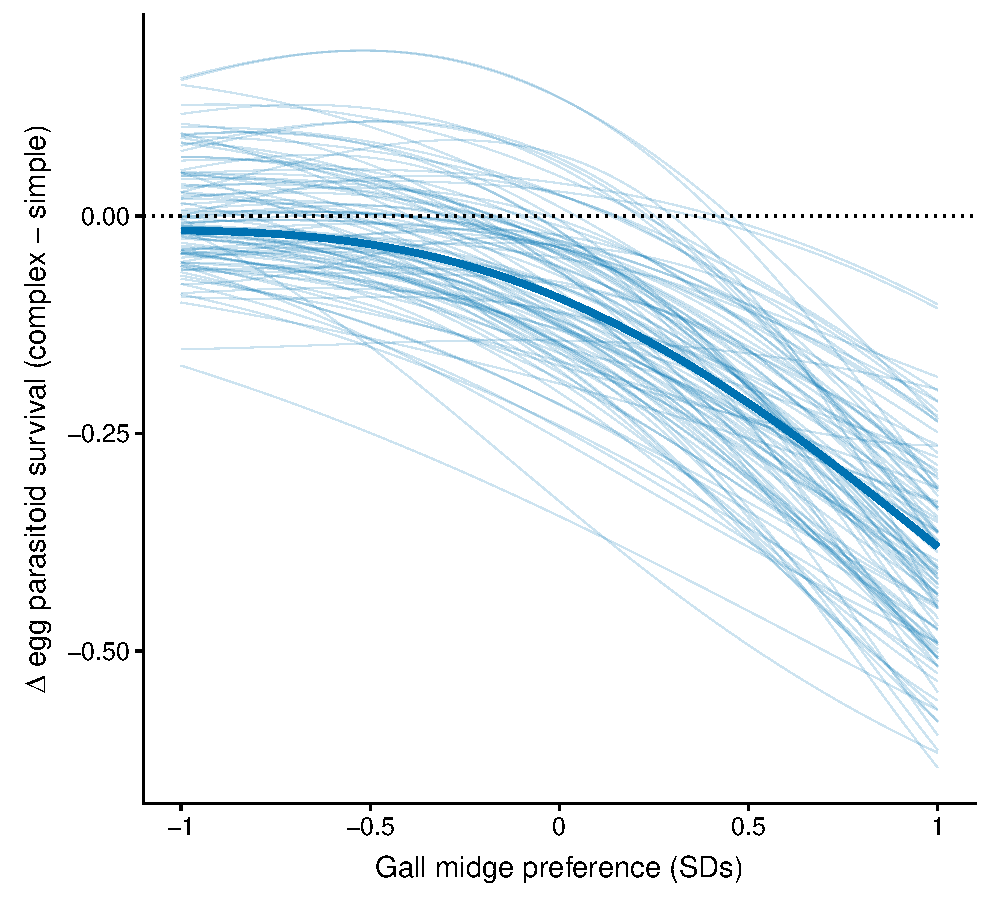
\includegraphics{../analyses/selection_on_Platygaster.pdf}
\caption{\label{fig:EggPtoid_Selection}Selection imposed by larval
parasitoids on egg parasitoids (\emph{Platygaster} sp.). The bold line
represents the average difference in the probability of observing the
egg parasitoid (original minus removal of larval parastioids) as a
function of gall midge oviposition preference. Thin lines represent
bootstrapped replicates to show the uncertainty in selection. For
clarity, we only display 100 bootstraps even though inferences are based
on 1,000 replicates. The decrease in the probability of observing egg
parasitoids at high gall-midge densities indicate that larval
parasitoids impose nonlinear selection on egg parasitoids.}
\end{figure}

\section{Discussion}\label{discussion}

We found that the removal of larval parasitoids constrained phenotypic
evolution in gall midges in two key ways. First, more traits contributed
to the slope of the adaptive landscape in the absence of larval
parasitoids, suggesting greater constraints on the trajectory of
phenotypic evolution. Second, excluding larval parasitoids altered the
curvature of the adaptive landscape in such a way that tended to
decrease the evolvability of associated traits. Assuming these traits
have other ecological functions, then this decrease in evolvability
could constrain the gall midge's adaptive potential in the face of novel
selection pressures. Our experiment also revealed evidence of indirect
selection pressures, suggesting that the loss of consumers may have
complex effects on the trajectories of phenotypic evolution. Taken
together, our study provides experimental evidence from the field that
the loss of consumers may constrain the adaptive potential of remaining
populations.

The generality of our results likely depends on the relative abundance
and functional differences between consumers in a community. For
example, if consumers do not differ from each other, then we do not
expect the loss of consumers to modify selective constraints. Also, many
consumers may be at too low of abundances to impose selection on their
resources. Rank abundance curves \citep{Preston1948} and the
disproportionate number of weak interactions in diverse communities
\citep{Paine1992} support this notion. This logic suggests that we may
not have observed the effects we did if we had only removed one larval
parasitoid, because each species had relatively low abundance
\citep{Barbour2016} and they likely share similar ecological roles. When
consumers are functionally different and abundant though, the effect of
consumer loss will depend on whether different species impose
conflicting selection pressures or select for distinct traits. When
consumers impose conflicting selection on traits, as in our study and
others \citep{Weis1985, Abrahamson1997, Start2016, Start2018}, then
consumer diversity acts to neutralize selection and relax selective
constraints. On the other hand, different consumers may impose selection
on different traits; therefore, a more diverse consumer community may
favor a particular combination of traits and increase selective
constraints. Examples of this include strong genetic covariances in
plant resistance to different insect herbivores
\citep{Maddox1990, Wise2007, Wise2013}, although there are also examples
where these covariances are weak \citep{Roche1997, Barbour2015}, or vary
from year-to-year \citep{Johnson2007}. We suggest that gaining
predictive insight to the evolutionary consequences of food-web
disassembly requires an understanding of the mechanisms governing the
assembly of trophic interactions \citep{Bascompte2009}.

We also found evidence for a general decrease in trait evolvability when
we excluded larval parasitoids due to changes in the curvature of the
adaptive landscape. This result was driven by nonlinear selection on
gall midge oviposition preference in the original food web, which was
due to both increases in intraguild predation and the lower mean
survival of gall midges. While these results are intriguing, they still
indicate that the indirect effects of selection are contingent on the
structure of a population's G-matrix (e.g.~consumer removals
\emph{increased} evolvability in 29\% of the scenarios). This highlights
the importance of future studies to characterize the G-matrix in order
to accurately predict how changes in network context will alter the
evolutionary potential of remaining populations. Indeed, current theory
often assumes genetic variances and covariances remain constant over
time rather than dynamically changing with the network context
\citep{McPeek2017, Guimaraes2017}. Our empirical results highlight the
need to explore the evolutionary consequences of not only direct effects
of selection, but indirect effects on genetic constraints that emerge in
a network of interacting species.

An important caveat of our study is that we did not due a factorial
manipulation of both parasitoid guilds, making it difficult to conclude
whether our results would change if we manipulated the presence/absence
of the dominant egg parasitoid. If we assume that higher-order
interactions \citep{Levine2017} are weak between parasitoid guilds, then
we can gain insight to how the loss of the egg parasitoid would alter
selection by isolating the contribution of larval parasitoids to
selection in our original food-web treatment. When we do this, we see
the same qualitative effects as we do when we removed larval
parasitoids. For example, we see clear evidence of all three traits
being under directional selection (i.e.~greater selective constraints,
Appendix A) as well as a decrease, albeit smaller, in trait evolvability
under different G-matrix scenarios (57\%, Appendix A). This suggests
that our results could be robust to this caveat, which was simply not
possible to manipulate given the biology of our system (see
\emph{Manipulating Food-web Structure} section for explanation).

Our results suggest that the loss of consumers may not only directly
affect connected species, but also result in indirect evolutionary
effects. In our study, this indirect effect arises from egg parasitoids
being released from intraguild predation when we excluded larval
parasitoids. This release occurs more on trees with high larval
densities, which could intensify future selection on gall midge
oviposition preference. A growing number of experiments over the past
two decades have demonstrated the presence and potential importance of
indirect evolutionary effects that emerge in ecological communities
\citep{Pilson1996, Juenger1998, Stinchcombe2001, Lankau2007, Walsh2008, Walsh2010, terHorst2010, Sahli2011, Lau2012, terHorst2015, Schiestl2018, Start2019}.
If indirect evolutionary effects are common
\citep{Miller1996, Walsh2013, Guimaraes2017}, then predicting
evolutionary trajectories resulting from the loss of consumers will
require evolutionary studies to explicitly account for the ecological
networks that species are embedded in.

Our study gives insight to how the loss of consumers alters evolutionary
constraints on remaining populations. In particular, it hints at a
potential insidious effect of local extinctions that compromises the
robustness of remaining populations to future environmental change. Our
work also highlights some key challenges for predicting phenotypic
evolution in rapidly changing communities. For example, many theoretical
models of eco-evolutionary dynamics focus on phenotypic change in a
single trait, yet our results highlight that the number of traits under
selection may change with the network context. Importantly, we found
that different species/guilds imposed different selection pressures.
Knowing these hidden selection pressures is critical for prediction,
because the trajectory of evolution will depend on the nature of change
in the ecological community. We expect that a continued integration of
adaptive landscapes and ecological networks will enhance our ability to
predict the evolutionary consequences of changes in ecological
communities.

\section{Acknowledgements}\label{acknowledgements}

We thank the staff of Humboldt Bay National Wildlife Refuge (U.S. Fish
and Wildlife Service) for facilitating experimental logistics. For
assistance with fieldwork, we thank Ruthie Espanol and Andrew MacDonald.
For funding support, we thank the University of British Columbia (James
Robert Thompson Fellowship and Four-Year Fellowship to M.A.~Barbour),
NSERC (Discovery grant to Greg Crutsinger), and the Swiss National
Science Foundation (grant 31003A\_160671 to J. Bascompte).

\section{Author Contributions}\label{author-contributions}

M.A.B. conceived the idea behind the study and designed the field
experiment. M.A.B. and B.L. setup and conducted the experiment. M.A.B.,
A.S., and C.J.G. collected the data. M.A.B. analyzed the data. M.A.B.
wrote the manuscript with primary input from J.B. and additional
feedback from C.J.G.

\section{Data Accessibility}\label{data-accessibility}

All data and code to reproduce the reported results are publicly
available on GitHub
(\url{https://github.com/mabarbour/complexity_selection}) and have been
archived on Zenodo (\url{https://zenodo.org/badge/latestdoi/108833263}).

\section{Appendix A}\label{appendix-a}

\bigskip

\begin{table}[h]
\caption{Standardized selection gradients acting on egg parasitoids (\textit{Platygaster} sp.)}
\label{Table:ExtendedGradients}
\centering
\begin{tabular}{lc}
\\ 
\hline
\textbf{Selection gradient} & \textbf{Contrast = Original - Removal}  \\ 
\hline
$\beta_{\text{Diam}}$ & 

-0.03 [
-0.3,
0.25] \\

$\beta_{\text{Clutch}}$ & 

0.07 [
-0.26,
0.39] \\

$\beta_{\text{Pref}}$ &

-0.25 [
-0.64,
0.09] \\

$\gamma_{\text{Diam:Diam}}$ &

-0.05 [
-0.43,
0.33] \\

$\gamma_{\text{Clutch:Clutch}}$ & 

-0.21 [
-0.68,
0.26] \\

$\gamma_{\text{Pref:Pref}}$ & 

\textbf{
-0.46 [
-1.07,
-0.02] }\\

$\gamma_{\text{Diam:Clutch}}$ & 

0 [
-0.29,
0.27] \\

$\gamma_{\text{Diam:Pref}}$ & 

0.25 [
-0.04,
0.6] \\

$\gamma_{\text{Clutch:Pref}}$ & 

-0.18 [
-0.52,
0.12] \\ 
\hline
\end{tabular}
\bigskip{}
\\
{\footnotesize Note: Values in brackets represent 95\% confidence intervals. Bold values indicate that the 95\% CI does not overlap zero. $\beta_{\text{Diam}}$ has been adjusted for bias.}
\end{table}

\bigskip

\begin{table}[h]
\caption{Standardized selection gradients imposed by larval parasitoids on gall midges in the original food web. This gives insight to selection acting on gall midges in the absence of the dominant egg parasitoid.}
\label{Table:LarvalGradients}
\centering
\begin{tabular}{lc}
\\ 
\hline
\textbf{Selection gradient} & \textbf{Larval Parasitoids} \\ % & \textbf{Original} 
\hline
$\beta_{\text{Diam}}$ & 
%\textbf{
%0.34 [
%0.22,
%0.48] } & 
\textbf{
0.23 [
0.13,
0.36] } \\

$\beta_{\text{Clutch}}$ & 
%0.06 [
%-0.05,
%0.17] & 
\textbf{
0.13 [
0.04,
0.24] }\\

$\beta_{\text{Pref}}$ &
%-0.13 [
%-0.29,
%0.05] & 
\textbf{
-0.17 [
-0.34,
-0.03] } \\

$\gamma_{\text{Diam:Diam}}$ &
%0.13 [
%-0.06,
%0.33] & 

0.06 [
-0.07,
0.2]  \\

$\gamma_{\text{Clutch:Clutch}}$ & 
%-0.05 [
%-0.27,
%0.18] & 

0.01 [
-0.14,
0.15] \\

$\gamma_{\text{Pref:Pref}}$ & 
%\textbf{
%0.34 [
%0.07,
%0.63] }& 

0.18 [
-0.02,
0.42] \\

$\gamma_{\text{Diam:Clutch}}$ & 
%-0.04 [
%-0.16,
%0.08] & 

0.02 [
-0.07,
0.11]  \\

$\gamma_{\text{Diam:Pref}}$ & 
%-0.13 [
%-0.29,
%0.02] & 

-0.05 [
-0.18,
0.06]  \\

$\gamma_{\text{Clutch:Pref}}$ & 
%0.03 [
%-0.1,
%0.18] & 

-0.04 [
-0.14,
0.06]  \\ 
\hline
\end{tabular}
\bigskip{}
\\
{\footnotesize Note: Values in brackets represent 95\% confidence intervals. Bold values indicate that the 95\% CI does not overlap zero. $\beta_{\text{Diam}}$ has been adjusted for bias.}
\end{table}

\begin{figure}
\centering
\includegraphics{../analyses/larvalptoid_delta_evolvability.pdf}
\caption{\label{fig:LarvalPtoidEvolvability}Change in average
evolvability for 10,000 random G-matrices using our best (mean) estimate
of the curvature matrix for selection in the absence of egg parasitoids
vs.~the original food web. We found that the curvature imposed by the
loss of egg parasitoids decreased evolvability in 57\% of the G-matrices
(i.e.~the change in evolvability was negative for 57\% of the
simulations), which is smaller in magnitude, but in the same direction,
as the effects of losing larval parasitoids.}
\end{figure}

\bibliography{references}


\end{document}
